% For instructions,
\documentclass[reprint, amsmath, amssymb, aps]{revtex4-2}

%\usepackage[norsk]{babel}
%Uncomment this if you want to write in Norwegian

\usepackage{graphicx}% Include figure files
\usepackage{dcolumn}% Align table columns on decimal point
\usepackage{bm}% bold math
\usepackage{hyperref}% add hypertext capabilities
\usepackage{booktabs}
\usepackage{float}
\usepackage{siunitx}



\begin{document}
\title{Project2 - FYS4460}
\author{Mikkel Metzsch Jensen}

\date{\today}
\maketitle

\subsection*{f) Diusion in a nano-porous material}
I have followed the description from question a-e. The lennard  fluid is first thermalized at $T = 0.851$ with a density corresponding to the unit cell length of 5.72 Å with fcc packing. We we measure the mean square displacement (msd) in the nano-porous material. The result is shown in figure \ref{fig:msd}.
\begin{figure}[H]
  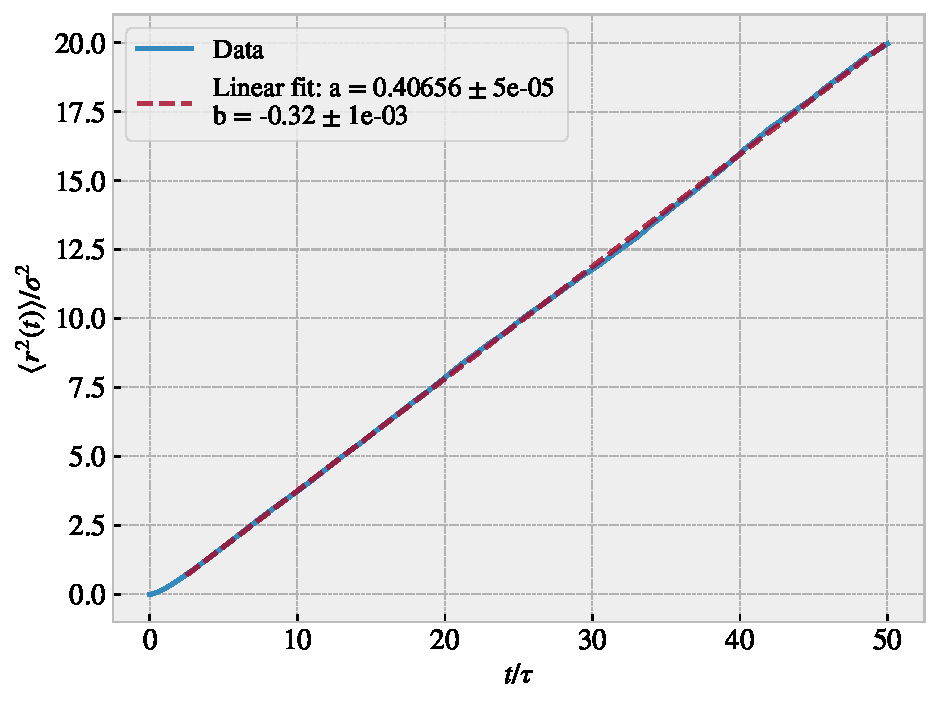
\includegraphics[width=\linewidth]{figures/msd.pdf}
  \caption{Mean square displacement $\langle r^2(t) \rangle$ as a function of time.}
  \label{fig:msd}
\end{figure}
We estimate the diffusion constant from the relaiton
\begin{align}
  \langle r^2(t) \rangle = 6Dt, \quad when \ t \rightarrow \infty
  \label{eq:diffusion}
\end{align}
From the linear fit on figure \ref{fig:msd} we estimate the diffusion constant  as
\begin{align*}
  D_{\text{nano-porus}} = \num{6.776e-2} \pm \num{8e-6}
\end{align*}



\subsection*{g) Flow in a nano porous material}

Darcy’s law is given as
\begin{align*}
  U = \frac{k}{\mu}(\nabla P - \rho g)
\end{align*}
Where $U$ is the volume flux (volume per area and time), $k$ is the permeability of the medium, $\mu$ is the viscosity, $\nabla P$ is the pressure drop over a given distance, $\rho$ is the density and $g$ is the gravitational acceleration. \par
We can relate the gravitional force as $F_G = mg$, thus we can rewrite the term $\rho g$ as
\begin{align*}
  \rho g = nmg = nF_G
\end{align*}
We can assume that gravity acts in x-direction such that $F_G = F_x$ and we get
\begin{align*}
  U = \frac{k}{\mu}(\nabla P - nF_x)
\end{align*}


\subsection*{h) Measure flow profile in pipe}

We use the same system consisting of $20 \times 20 \times 20$ unit boxes and carve out a cylinder along the x-axis with radius 12 Å. Everything outisde the cylinder is frozen while the atoms inside can move freely. The freely moving atoms is reduced to half density. We add a force $F_x = 0.1 \ \epsilon/\sigma$ on every free atom in the x-direction. We then let the system stabilize and measure the flow profile, that is the velocity in x-direction as a function of radial distace to the x-axis. \par
We run the simulations for almost 450 $\tau$ (the simulation suddently crashed at this point). We calculate the innerproduct for the velocity distribution as
\begin{align}
  \frac{\sum_i h_i(t)h_i(t_n)}{\sum_i h_i(t_n)^2}
  \label{eq:inner_product}
\end{align}
where $h_i$ is the height of radial bin $i$ in the histogram and $t_n$ is the final time-step. We then plot this to confirm that the cistirbution is converging towards a steady state (see figure \ref{fig:flow_inner_product}).
\begin{figure}[H]
  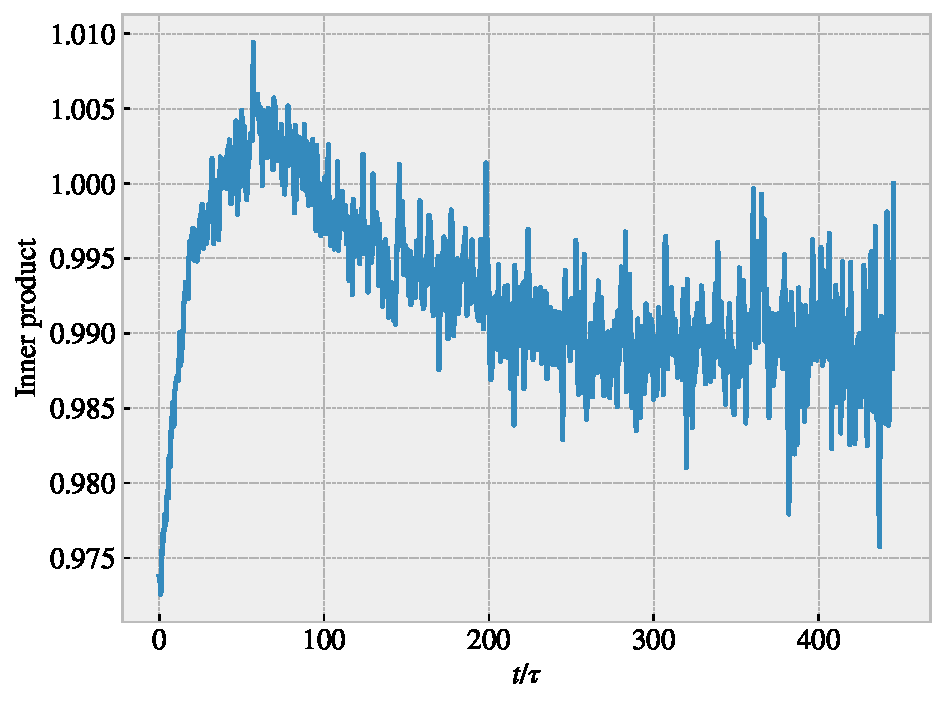
\includegraphics[width=\linewidth]{figures/flow_inner_product.pdf}
  \caption{The inner product (equation \ref{eq:inner_product}) for the velocity distribution $v_x(r)$ with radial bins. We see that the distirbution is somewhat reaching a steady state towards the end. We also notice bigger fluctuations which can probably be connected to the crash of the simmulaitons at the end.}
  \label{fig:flow_inner_product}
\end{figure}
Theoretically we expect the flow profile to follow:
\begin{align*}
  u(r) = \frac{G}{4\mu}(R^2 - r^2)
\end{align*}
(equation 4.27 in \cite{compendium}), where $R$ is the radius of the cylinder and $G = |\Delta P|/L$ with
\begin{align*}
  \Delta P = p_1 - p_2 = \rho g (h_1 - h_2) - \rho g L
\end{align*}
(equation 6.2 in \cite{compendium}). Since we have no height difference in this system we only have a contribution from the hydrostatic pressure $\rho gL$. In addition we swapped the gravity with the force $F_x$ and we get
\begin{align*}
  G = |-\frac{nF_xL}{L}| = nF_x
\end{align*}
From this we expect the flow profile in x-direction to follow the relation:
\begin{align}
  v_x(r) = \frac{nF_x}{4\mu}(R^2 - r^2)
  \label{eq:v_x}
\end{align}
By making a linear fit between $y = v_x(r)$ and $x = (R^2 - r^2)$ we can estimate the value $\frac{nF_x}{4\mu}$ as the slope on the fit $a$ as shown in figure \ref{flow_profile_linfit}
\begin{figure}[H]
  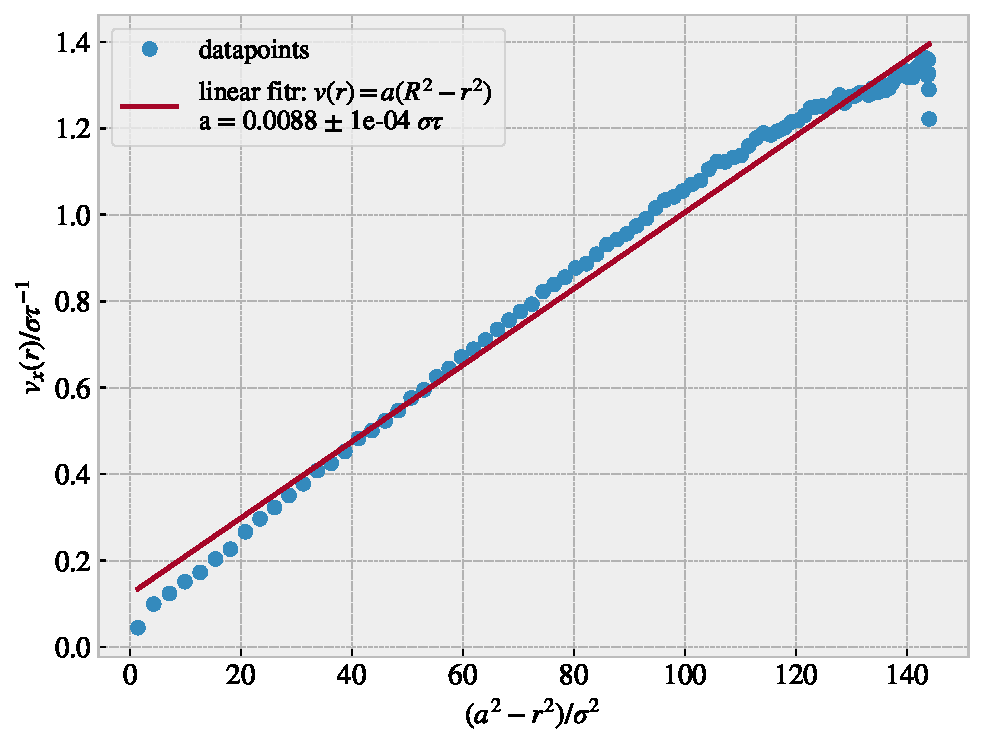
\includegraphics[width=\linewidth]{figures/flow_profile_linfit.pdf}
  \caption{Linear fit from relation \ref{eq:v_x}.}
  \label{fig:flow_profile_linfit}
\end{figure}
The actual profile is shown along side with the fit in figure \ref{fig:flow_profile}
\begin{figure}[H]
  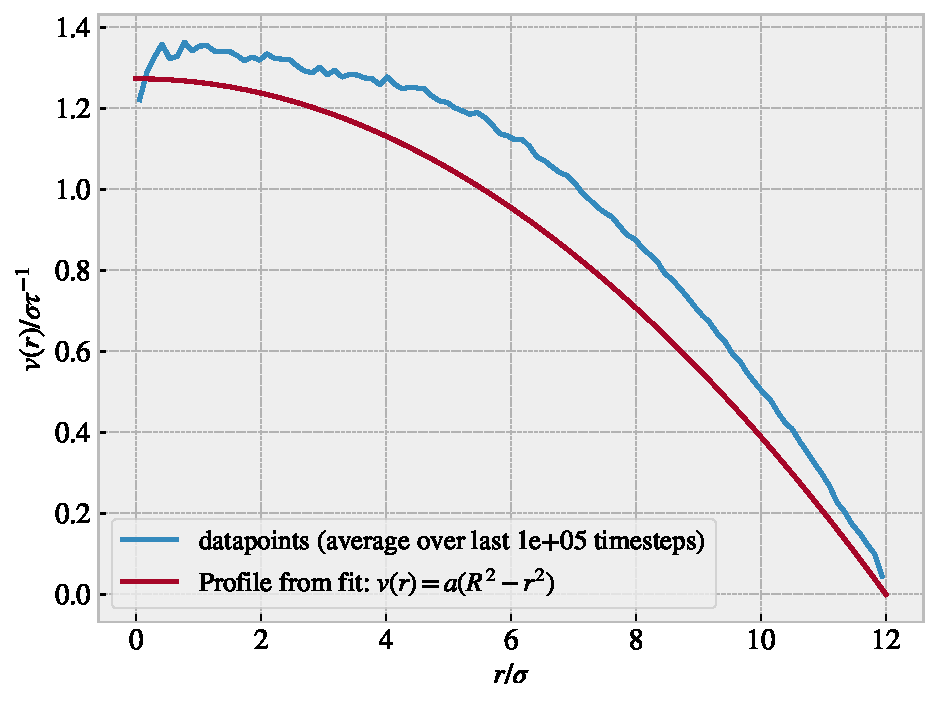
\includegraphics[width=\linewidth]{figures/flow_profile.pdf}
  \caption{Expermental and fitted velocity profile.}
  \label{fig:flow_profile}
\end{figure}

From the fit shown in figure \ref{fig:flow_profile_linfit} we estimate the viscosity $\mu$ to be
\begin{align*}
  \mu = \frac{n F_x}{4a} = 1.19 \pm 0.01
\end{align*}







\begin{thebibliography}{9}
\bibitem{compendium}
Jens Feder, Flow in Porous Media
\end{thebibliography}

\end{document}
